\documentclass[a4paper]{report}
\usepackage[spanish]{babel}
\selectlanguage{spanish}
\usepackage[utf8]{inputenc}
\usepackage[T1]{fontenc}
\usepackage{pdfpages}
\usepackage[a4paper,top=2cm,bottom=2cm,left=2cm,right=2cm]{geometry}
\usepackage{amsmath, amsthm, amsfonts}
\usepackage{graphicx}
\usepackage{minitoc}
\usepackage{color}
\usepackage{listings}
\usepackage{hyperref}
\usepackage{multicol}

\hypersetup{
    colorlinks=true, % make the links colored
    linkcolor=black, % color TOC links in blue
    urlcolor=red, % color URLs in red
    linktoc=all % 'all' will create links for everything in the TOC
}

\lstset{
basicstyle=\ttfamily,
captionpos=b,
frame=single
}

\def\blankpage{%
      \clearpage%
      \thispagestyle{empty}%
      \addtocounter{page}{0}%
      \null%
      \clearpage}
    
\title{Desarrollo de la Lógica Proposicional y de Primer Orden bajo el paradigma funcional y la orientación Web.}
\author{Víctor Ramos González\\\\
   Tutor: Fernando Sancho Caparrini\\
   \textit{Ciencias de la Computación e Inteligencia Artificial}\\
   E.T.S. Ingeniería Informática\\
   Universidad de Sevilla\\
  \vspace{8cm}
  \date{Septiembre 2020}
}

\setlength{\parskip}{1em} 
 
\sloppy
\begin{document}

\dominitoc

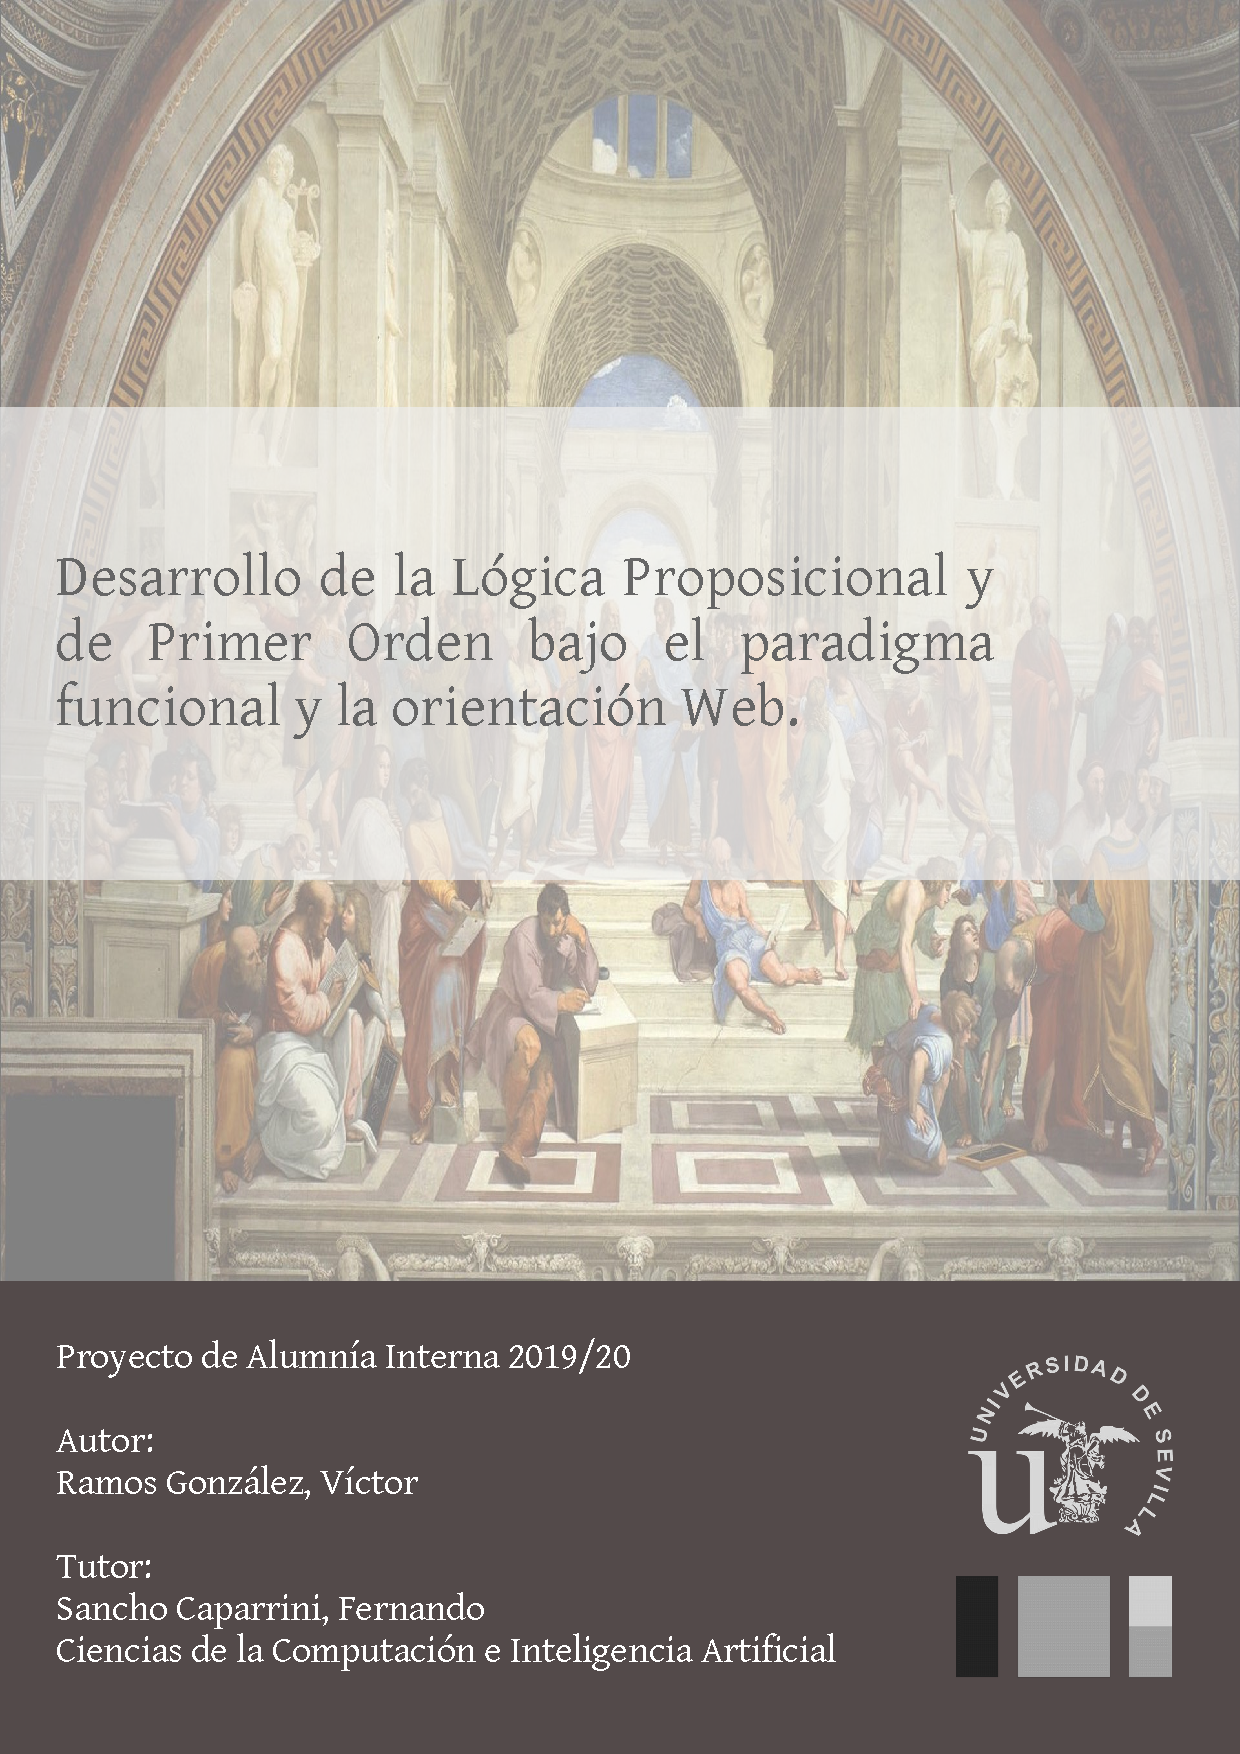
\includepdf[pages={1}]{archivos/titlepage.pdf}


\blankpage

\maketitle

\begin{abstract}

El proyecto aborda los conceptos y algoritmos básicos de la Lógica Proposicional y la Lógica de primer, desde un punto de vista implementativo a través de un lenguaje encuadrado en el paradigma funcional (Elm).

El proyecto, basado en la asignatura de Lógica Informática, busca una doble finalidad, por un lado servir como una somera introducción a la programación declarativa al mismo que tiempo que proporcionar al alumnado  herramientas intuitivas y de sencillo uso en la realización de los ejercicios que apoyen los contenidos teóricos que se desarrollan en dicha asignatura.
\end{abstract}

\tableofcontents

\newpage


\chapter{Introducción. Objetivos y organización del proyecto}
\renewcommand{\mtctitle}{}
\mtcskip
\minitoc
\newpage

\section{Introducción}

Tras haber cursado la asignatura de Lógica Informática con el profesor D. Fernando Sancho Caparrini, director de este proyecto, se despertó mi gusto por la Teoría de la Lógica Matemática y Computacional. Aunque desde el punto de vista teórico la asignatura presentaba los contenidos de forma completa y con total formalismo y corrección, los profesores encargados de la misma pretendían darle a la misma un enfoque más práctico de manera que estos nuevos contenidos sirvieran como complemento a los conceptos formales presentados teóricamente.


\section{Objetivos del proyecto}
El proyecto persigue un doble objetivo,

\section{Estructura del proyecto}

El proyecto se estructará en 2 partes fundamentales:

\subsection{Módulos funcionales}

Se implementan distintos módulos, que se describen detalladamente a lo largo del proceso, en el que se desarrollarán las estructuras y métodos necesarios para abordar los algoritmos vistos en la asignatura.

\subsection{Interfaz gráfica}

\chapter{LP I. Sintaxis y Semántica}
\renewcommand{\mtctitle}{}
\mtcskip
\minitoc
\newpage
\section{Introducción. Descripción general del capítulo}

\textit{TO DO}

\newpage
\section{Módulo SintaxSemanticsLP}

En este primer capítulo vamos a estudiar, desde un punto de vista práctico, a través de las implementaciones, los distintos elementos que conforman la Lógica Proposicional, esto es la Síntaxis y la Semántica que se han presentado en los fundamentos teóricos.

\subsection{Aspectos Sintácticos}

\subsubsection{Átomo y Fórmula Proposicional}

Recordemos que las expresiones están formadas por símbolos proposicionales, organizados en átomos (expresiones básicas) y relaciones entre ellas (conectivas), de acuerdo a esto, podemos definir un símbolo proposicional como una cadena de texto:\\

\begin{lstlisting}[caption= Definición de Símbolo Proposicional como alias de String.]
type alias PSymb = String 
\end{lstlisting}

Y las conectivas lógicas como categorías del tipo recursivo \textit{Prop}, de forma que:\\

\begin{lstlisting}[caption= Definición del tipo Prop (Proposición).]
type Prop = Atom PSymb
          | Neg Prop
          | Conj Prop Prop
          | Disj Prop Prop
          | Impl Prop Prop
          | Equi Prop Prop
\end{lstlisting}

Esto nos permite definir todas las fórmulas proposicionales que se pueden formar, algunos ejemplos: \\

\begin{multicols}{3}
\begin{itemize}
\item[(a)] $ (p \wedge q) \vee (p \wedge r)$
\item[(b)] $ (p \wedge r) \vee (\neg p \wedge q) \rightarrow \neg q$
\item[(c)] $(p \leftrightarrow q) \wedge (p \rightarrow \neg q) \wedge p$
\end{itemize}
\end{multicols}

\begin{lstlisting}[caption= Ejemplos de definición de fórmulas proposicionales.]
a = Disj (Conj (Atom "p") (Atom "q")) (Conj (Atom "p") (Atom "r"))
    
b = Impl 
        (Disj 
            (Conj (Atom "p") (Atom "r")) 
            (Conj (Neg (Atom "p")) (Atom "q"))
        ) 
        (Neg (Atom "q"))

c = Conj 
        (Conj 
            (Equi (Atom "p") (Atom "q")) 
            (Impl (Atom "p") (Neg (Atom "q"))) 
        (Atom "p")
\end{lstlisting}

Como se puede apreciar, escribir las fórmulas de esta forma puede resultar una tarea ardua y propensa a errores, por eso, como mostraremos más adelante, se ha desarrollado un parser que nos permite escribir de forma más cómoda, sintética y visual las fórmulas. Aunque aquí no influyen las reglas de asociación vistas en los fundamentos teóricos, ya que dicho orden viene dado por el propio orden de aplicación, sí hemos de tenerlas en cuenta a la hora de realizar el parser. 

\subsubsection{Conjuntos de fórmulas}

Definidas las fórmulas proposicionales, definiremos los conjuntos de fórmulas como listas de fórmulas proposicionales de manera que una misma fórmula puede aperecer varias veces en el conjunto. De esta forma: \\

\begin{lstlisting}[caption= Definición de Conjunto de Fórmulas como Lista de Fórmulas Proposicionales]
type alias PropSet = List Prop
\end{lstlisting}

\subsection{Aspectos Semánticos}
\subsubsection{Interpretaciones y Valor de verdad de fórmulas proposicionales. }

Una vez provista la sintaxis, pasamos a desarrollar la semántica de la Lógica Proposicional. Aunque en secciones futuras mostraremos la implementación del parser, por ahora vasta conocer la estructura de las fórmulas para hacer abordable la implementación que se ha llevado a cabo de la semática del lenguaje de la lógica de proposiciones.

Como ya se ha comentado, y explicado en los fundamentos teóricos, hemos de abordar la interpretación de las fórmulas, y para ello hemos de crear las estructuras necesarias que nos permitan representar interpretaciones, esto es, definir los símbolos proposicionales con valor de verdad 1 y aquellos con valor 0. Para ello, hemos elegido una representación "dispersa" de manera que una interpretación corresponde a una lista de símbolos proposicionales que son los que son considerados verdaderos, los términos que no aparecen en la lista serán considerados como falsos.\\

\begin{lstlisting}[caption= Definición de Interpretación como Lista de Símbolos Proposicionales]
type alias Interpretation = List PSymb
\end{lstlisting}

De esta forma podemos definir, de forma sencilla la evaluación de las fórmulas, de forma que el valor de verdad de un símbolo se reduce a la pertenencia del mismo a la lista de interpretación, de esta forma, podemos, dada la estructura recursiva definida para las fórmulas proposicionales, establecer una función, tambieén recursiva, que nos permite evaluar las mismas:

\begin{itemize}
\item (\textit{Caso base}) Una fórmula atómica será verdadera si y sólo si el símbolo proposicional pertenece a la lista de interpretación.

\item (Casos recursivos) Según la clase de fórmula:
\begin{itemize}
\item La negación de una fórmula será verdadera respecto de una interpretación si y sólo si la evaluación de la fórmula es falsa.
\item La conjunción de dos fórmulas proposicionales será verdadera respecto de una interpretación si y sólo si la evaluación de ambas fórmulas respecto de dicha evaluación es verdadera.
\item La disyunción de dos fórmulas proposicionales será verdadera será verdadera respecto de una interpretación si y sólo si alguna de las evaluaciones de las dos fórmulas es evaluada verdadera respecto de dicha interpretación.
\item La implicación será verdadera respecto de una interpretación si y sólo si o la evaluación del antecedente es evaluado falso respecto de dicha interpretación o el consecuente es evaluado verdadero respecto de la misma.
\item La equivalencia será verdadera respecto de una interpretación si y sólo si la evaluación del antecedente coincide con la evaluación del consecuente.\\
\end{itemize} 

\newpage
\begin{lstlisting}[caption= Función de evaluación de las fórmulas proposicionales]
valuation : Prop -> Interpretation -> Bool
valuation pr i =
    case pr of
        Atom p -> List.member p i
        Neg p -> not (valuation p i)
        Conj p q -> valuation p i &&  valuation q i
        Disj p q ->   valuation p i ||  valuation q i
        Impl p q ->   not (valuation p i) ||  valuation q i
        Equi p q ->   valuation (Impl p q) i &&  valuation (Impl q p) i
\end{lstlisting}
\end{itemize}

\subsubsection{Modelos (tablas de verdad, satisfactibilidad y validez lógica)}

Desde el punto de vista teórico las tablas de verdad corresponden a estructuras que reflejan el valor de verdad de una fórmula proposicional respecto de cada una de las posibles interpretaciones posibles para la fórmula. Entonces, para poder construir la tabla de verdad, primero hemos de calcular todas las interpretaciones posibles, que, dada la definición que hemos proporcionado para las interpretaciones, correspondería a todos los conjuntos posibles (\textit{powerset}) que podríamos construir con los símbolos proposicionales que aparecen en la fórmula. Así:\\

\begin{lstlisting}[caption= Función para extraer los símbolos proposicionales que intervienen en una fórmula]
symbInProp : Prop -> Set PSymb

symbInProp f=
    case f of
        Atom p -> Set.singleton p
        Neg p -> symbInProp p
        Conj p q -> Set.union (symbInProp p ) (symbInProp q)
        Disj p q -> Set.union (symbInProp p ) (symbInProp q)
        Impl p q -> Set.union (symbInProp p ) (symbInProp q)
        Equi p q -> Set.union (symbInProp p ) (symbInProp q)
\end{lstlisting}

\begin{lstlisting}[caption= Función para extraer las posibles interpretaciones para una fórmula propsicional]
allInterpretations : Prop -> List Interpretation
allInterpretations x =  Aux.powerset <| List.sort <| Set.toList 
                                                         <| symbInProp x
\end{lstlisting}

De esta forma podemos expresar la tabla de verdad como una lista de tuplas en las que el primer elemento corresponde a la interpretación y el segundo corresponde a la evaluación de la fórmula respecto de dicha valoración:\\

\begin{lstlisting}[caption= Función para la construcción de la tabla de verdad de una fórmula]
truthTable : Prop -> List (Interpretation, Bool)
truthTable x = List.map (\xs ->  (xs,valuation x xs)) <| allInterpretations x
\end{lstlisting}

Una vez estudiado lo anterior, los modelos corresponden a las interpretaciones que son evaluadas verdaderas, esto es, de las posibles interpretaciones aquellas hacen la fórmula verdadera. Aquellas interpretaciones que hacen la fórmula falasa se denominan contramodelos. Así:\\

\newpage
\begin{lstlisting}[caption= Función para el cálculo de los modelos de una fórmula proposicional]
models : Prop -> List Interpretation
models x = List.filter (\y -> valuation x y) (allInterpretations x)

countermodels : Prop -> List Interpretation
countermodels x = List.filter (\y -> not (valuation x y)) 
                                               (allInterpretations x)
\end{lstlisting}

Definidos los modelos, podemos así mismo definir (funcionalmente) los conceptos de satisfactibilidad y validez, de forma que:

\begin{itemize}
\item Una fórmula es satisfactible si posee al menos un modelo.
\item Una fórmula es lógicamente válida o tautología si toda interpretación es modelo de la fórmula.
\item Una fórmula es insatisfactible o contradicción si no posee ningún modelo.
\end{itemize}

De esta forma:

\begin{lstlisting}[caption={Funciones de Satisfactibilidad, Validez e Insatisfactibilidad}]
satisfactibility : Prop -> Bool
satisfactibility x = List.any (\xs-> valuation x xs) (allInterpretations x)

validity : Prop -> Bool
validity x = List.all (\xs-> valuation x xs) (allInterpretations x)

insatisfactibility : Prop -> Bool
insatisfactibility x = not (satisfactibility x)
\end{lstlisting}

\subsubsection{Conjuntos de Fórmulas. Modelos, Consistencia, Validez y Consecuencia Lógica}

Vista la satisfactibilidad, modelos, etc. aplicadas a una fórmula, pasamos a desarrollar los métodos necesarios para el estudio de la satisfactibilidad (consistencia) , inconsistencia en conjuntos de fórmulas. Ahora los modelos del conjunto de fórmulas corresponden a las interpretaciones tales que hacen verdaderas todas las fórmulas del conjunto. Para obtener los modelos hemos, al igual que en el caso de las fórmulas, obtener el conjunto de símbolos proposicionales y a partir de estos el conjunto de todas las posibles interpretaciones. De forma que:\\

\begin{lstlisting}[caption={Modelos y contramodelos en conjuntos de fórmulas proposicionales}]
setSymbols : List Prop -> Set PSymb
setSymbols xs = 
    List.foldr (\x acc -> Set.union acc (symbInProp x)) Set.empty xs

allSetInterpretations : List Prop -> List Interpretation
allSetInterpretations xs = Aux.powerset <| Set.toList <| setSymbols xs
    
isSetModel : List Prop -> Interpretation -> Bool
isSetModel xs i =  List.all (\x -> valuation x i) xs

allSetModels : List Prop -> List Interpretation
allSetModels xs = List.filter (isSetModel xs) (allSetInterpretations xs)

allSetCounterModels : List Prop -> List Interpretation
allSetCounterModels xs = 
    List.filter (\x -> not(isSetModel xs x)) <| allSetInterpretations xs
\end{lstlisting}


De forma que ahora, es sencillo, comprobar la consistencia de un conjunto a partir de la definición: \textit{`Un conjunto es consistente si posee, al menos, un modelo. En caso contrario es inconsistente'}\\

\begin{lstlisting}[caption={Consistencia e Inconsistencia en Conjuntos Proposicionales}]
isConsistent : List Prop -> Bool
isConsistent xs = 
    List.any (\x -> isSetModel xs x) <| allSetInterpretations xs
    
isInconsistent: List Prop -> Bool
isInconsistent xs = not(isConsistent xs)
\end{lstlisting}

Por último nos queda definir el concepto de consecuencia lógica. Acudiendo a la definición: \textit{`Una fórmula es consecuencia lógica de un conjunto de fórmulas si y sólo si todo modelo del conjunto es también modelo de la fórmula'}, pero también \textit{`Una fórmula es consecuencia lógica de un conjunto de fórmulas si la unión del conjunto y el conjunto formado por la negación del la fórmula es inconsistente.'}. De esta forma podemos plantear dos desarrollos alternativos:\\

\begin{lstlisting}[caption={Consecuencia Lógica}]
isConsecuence : List Prop -> Prop -> Bool
isConsecuence xs x = List.all (\y -> valuation x y) <| allSetModels xs

isConsecuence : List Prop -> Prop -> Bool
isConsecuence xs x = isInconsistent (xs ++ [Neg x])
\end{lstlisting}

\subsection{Código del módulo y resumen de funciones}

\section{Módulo LP\_toString}


\section{Módulo A\_Expressions (Expr. Aritméticas)}
\section{Módulo B\_Expressions (Expr. Booleanas)}
\section{Módulo LP\_Parser}
\section{Módulo LPBig\_Parser}

\chapter{LP II. Tableros Semánticos}
\renewcommand{\mtctitle}{}
\mtcskip
\minitoc
\newpage
\chapter{LP III. Formas Normales y DPLL}
\renewcommand{\mtctitle}{}
\mtcskip
\minitoc
\newpage
\chapter{LP IV. Sistemas Deductivos}
\renewcommand{\mtctitle}{}
\mtcskip
\minitoc
\newpage
\chapter{LP V. Algoritmo de Resolución}
\renewcommand{\mtctitle}{}
\mtcskip
\minitoc
\newpage
\chapter{LP VI. Modelado y Resolución de PSR a través de la LP}
\renewcommand{\mtctitle}{}
\mtcskip
\minitoc
\newpage

\chapter{LPO I. Sintaxis y Semántica}
\renewcommand{\mtctitle}{}
\mtcskip
\minitoc
\newpage
\chapter{LPO II. Tableros Semánticos}
\renewcommand{\mtctitle}{}
\mtcskip
\minitoc
\newpage
\chapter{LPO III. Forma Prenex, Skolem y Teorema de Herbrand}
\renewcommand{\mtctitle}{}
\mtcskip
\minitoc
\newpage
\chapter{LPO V. Algoritmos de Unificación y Resolución}
\renewcommand{\mtctitle}{}
\mtcskip
\minitoc
\newpage
\chapter{LPO VI. Modelado y Resolución de PSR a través de la Lógica de Primer Orden}
\renewcommand{\mtctitle}{}
\mtcskip
\minitoc
\newpage

\end{document}